\documentclass{beamer}
\usepackage[british,spanish]{babel}
\usepackage[utf8]{inputenc}
\usepackage{hyperref}
\usepackage{multirow}



\usepackage{listings}

\usepackage{adjustbox}
\usepackage{lstcustom}

\usepackage{color}
\definecolor{light-gray}{gray}{0.80}
\definecolor{lstbackgroundshellcolor}{named}{light-gray}

\usepackage{tikz}
\newcommand*\circled[1]{\tikz[baseline=(char.base)]{
            \node[shape=circle,draw,inner sep=2pt] (char) {#1};}}

\usepackage[normalem]{ulem}

%\usepackage[acronym,xindy,toc]{glossaries}

\usepackage[acronym,xindy,toc]{glossaries}
\makeglossaries
%\usepackage[xindy]{imakeidx}
%\makeindex

\newcommand{\comment}[2]{#2}

\graphicspath{ {./images/} }

\title[Cloud Computing with Amazon Web Services]{Cloud Computing with Amazon Web Services}
%\subtitle[short subtitle]{long subtitle}
\author[C. Cuenca, F. Quintana]{Carmelo Cuenca-Hernández and Francisca Quintana-Domínguez}
%\institute{Escuela Universitaria de Informática}
%\date[04/2013]{Abril - 2013}
\date{}
\titlegraphic{
\includegraphics[width=0.5 \textwidth]{images/awslogo.eps}}



\pgfdeclareimage[width=2.0\baselineskip]{ulpgc-logo}{images/logosimbolo_secundario_version_vertical}
\setbeamertemplate{footline}{\raisebox{-2ex}{\pgfuseimage{ulpgc-logo}}
  \usebeamerfont{date in head/foot}\insertshortdate{}\hfill
  \usebeamertemplate{navigation symbols}\hfill
  \insertframenumber{}/\inserttotalframenumber}
\setbeamertemplate{sidebar right}{}


\usetheme{Antibes}
%\usetheme{Berlin}

%\usetheme{Warsaw}
%\usecolortheme{albatross}

\begin{document}

\begin{frame}
	\titlepage
\end{frame}


\section*{Outline}
\begin{frame}
  \frametitle{Outline}
  %\tableofcontents%[part=1,pausesections]
  \tableofcontents[currentsection,currentsubsection, sectionstyle=show] 
  %\tableofcontents[currentsection,sectionstyle=show,hideothersubsections]
\end{frame}


\selectlanguage{british}

%%%%%%%%%%%%%%%%%%%%%%%%%%%%%%%%%%%%%%%%%%%%%%%%%%%%%%%%%%%%%%%%%%%%%%%%%%%%%%
%\newacronym{<label>}{<abbrv>}{<full>}
%\glsreset{<label>}
%\glsresetall
%\acrlong{<label>}
%\acrfull{<label>}
%\acrshort{<label>}
\newacronym{aws}{AWS}{Amazon Web Services}
\newacronym{ebs}{EBS}{Elastic Block Storage}
\newacronym{ec2}{EC2}{Amazon Elastic Compute Cloud}
\newacronym{ecu}{ECU}{Elastic Compute Unit}
\newacronym{elb}{ELB}{Elastic Load Balancing}
\newacronym{rds}{RDS}{Relational Database Service}
\newacronym{s3}{S3}{Simple Storage Service}
\newacronym{sqs}{SQS}{Amazon Simple Queue Service}
%%%%%%%%%%%%%%%%%%%%%%%%%%%%%%%%%%%%%%%%%%%%%%%%%%%%%%%%%%%%%%%%%%%%%%%%%%%%%%
\section[Amazon Web Services]{Amazon Web Services}
%%%%%%%%%%%%%%%%%%%%%%%%%%%%%%%%%%%%%%%%%%%%%%%%%%%%%%%%%%%%%%%%%%%%%%%%%%%%%%
\begin{frame}
\frametitle{Amazon Web Services}
\begin{figure}
  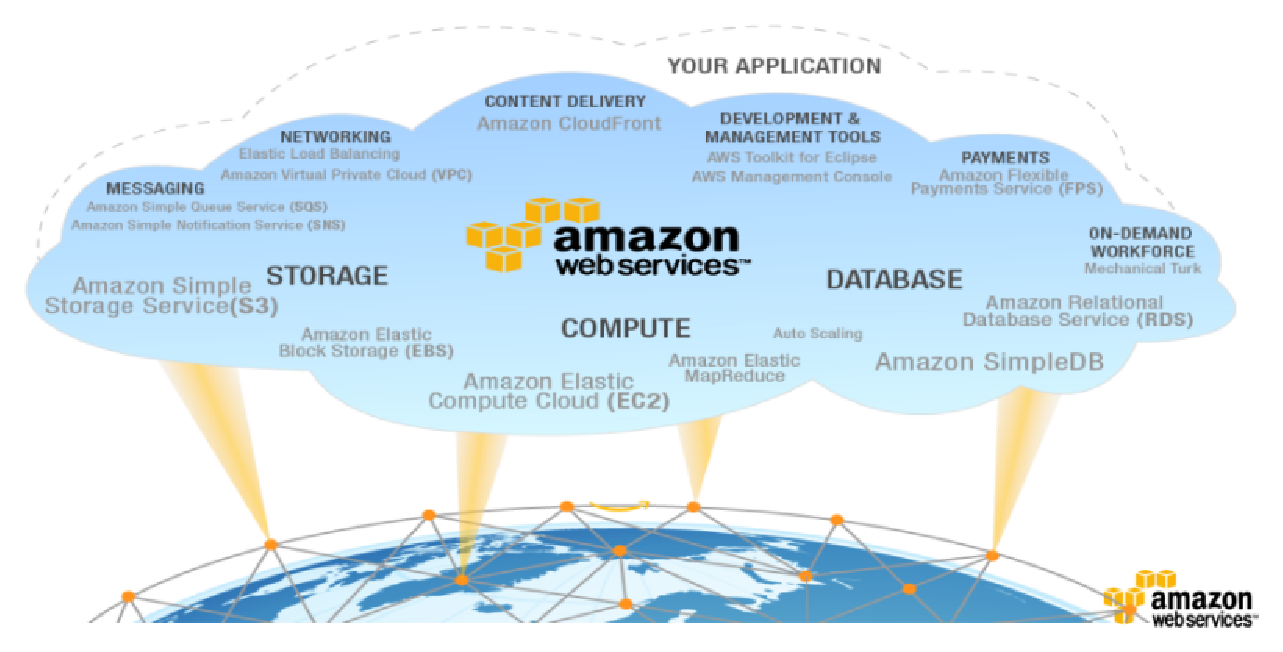
\includegraphics[width= 1.0 \textwidth]{infraestructura-tecnologica-de-amazon-web-services-para-brindar-servicios-cloud-saas-iaas-y-paas.eps}
\end{figure}
\end{frame}
%%%%%%%%%%%%%%%%%%%%%%%%%%%%%%%%%%%%%%%%%%%%%%%%%%%%%%%%%%%%%%%%%%%%%%%%%%%%%%
\begin{frame}
\frametitle{Amazon Web Services}
\begin{itemize}
 \item Storage \& Content Delivery
  \begin{itemize}
    \item \gls{s3}
    \item \gls{ebs}
    \item Amazon CloudFront
  \end{itemize}  
\item Compute \& Networking
  \begin{itemize}
    \item \gls{ec2}
    \item Auto Scaling
    \item \gls{elb}
  \end{itemize}
  \item Database
  \begin{itemize}
    \item \gls{rds}
    \item Amazon Simple Database (SimpleDB)
  \end{itemize}
  \item Deployment \& Management
  \begin{itemize}
    \item Amazon CloudWatch
  \end{itemize}
  \item App Services
  \begin{itemize}
    \item \gls{sqs}
  \end{itemize}
\end{itemize}
\end{frame}


%%%%%%%%%%%%%%%%%%%%%%%%%%%%%%%%%%%%%%%%%%%%%%%%%%%%%%%%%%%%%%%%%%%%%%%%%%%%%%
\begin{frame}
\frametitle{Dollars and Cents}
\begin{itemize}
\item \gls{aws} is a pay-as-you-go web service, there's separate cost for use of each service
\item We can also use the \gls{aws} Simple Monthly Calculator
\url{http://calculator.s3.amazonaws.com/calc5.html}
\end{itemize}
\end{frame}
%%%%%%%%%%%%%%%%%%%%%%%%%%%%%%%%%%%%%%%%%%%%%%%%%%%%%%%%%%%%%%%%%%%%%%%%%%%%%%
\begin{frame}
\frametitle[\gls{s3}]{\acrfull{s3}}
\url{https://aws.amazon.com/s3/}
\begin{columns}
  \column{0.60 \textwidth}
  \begin{itemize}
  \item It gave everyone access to an ultra-reliable and highly scalable storage service without having to invest tens of thousands of dollars for an exclusive enterprise storage solution
  \item The service sat directly on the Internet, and objects were directly HTTP addressable
  \end{itemize}
  \column{0.40 \textwidth}
  \begin{figure}
	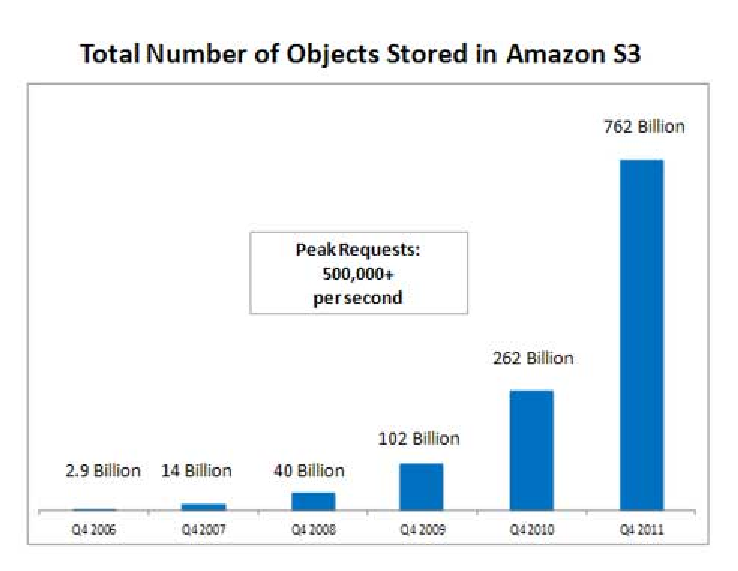
\includegraphics[width= 1.0 \textwidth]{aws-s3-growth.eps}
  \end{figure}
\end{columns}
\end{frame}


%%%%%%%%%%%%%%%%%%%%%%%%%%%%%%%%%%%%%%%%%%%%%%%%%%%%%%%%%%%%%%%%%%%%%%%%%%%%%%
\begin{frame}
\frametitle[\gls{ebs}]{\acrfull{ebs}}
\url{https://aws.amazon.com/ebs/}

  Amazon \gls{ebs}
  \begin{itemize}
  \item provides block level storage volumes for use with \gls{ec2} instances
  \item volumes are network-attached, and persist independently from the life of an instance
  \item provides highly available, highly reliable, predictable storage volumes that can be attached to a running \gls{ec2} instance and exposed as a device within the instance
  \item particularly suited for applications that require a database, file system, or access to raw block level storage.
  \end{itemize}
\end{frame}


%%%%%%%%%%%%%%%%%%%%%%%%%%%%%%%%%%%%%%%%%%%%%%%%%%%%%%%%%%%%%%%%%%%%%%%%%%%%%%
\begin{frame}
\frametitle[CloudFront]{CloudFront}
\begin{columns}
\column{0.65 \textwidth}
\url{http://aws.amazon.com/cloudfront/}
 Amazon CloudFront
\begin{itemize}
  \item is a web service for content delivery
  \item can be used to deliver dynamic, static and streaming content using a global network of edge locations
  \item is optimized to work with other \Gls{aws}, like \gls{s3}, \gls{ec2} and \gls{elb}
\end{itemize}
\column{0.35 \textwidth}
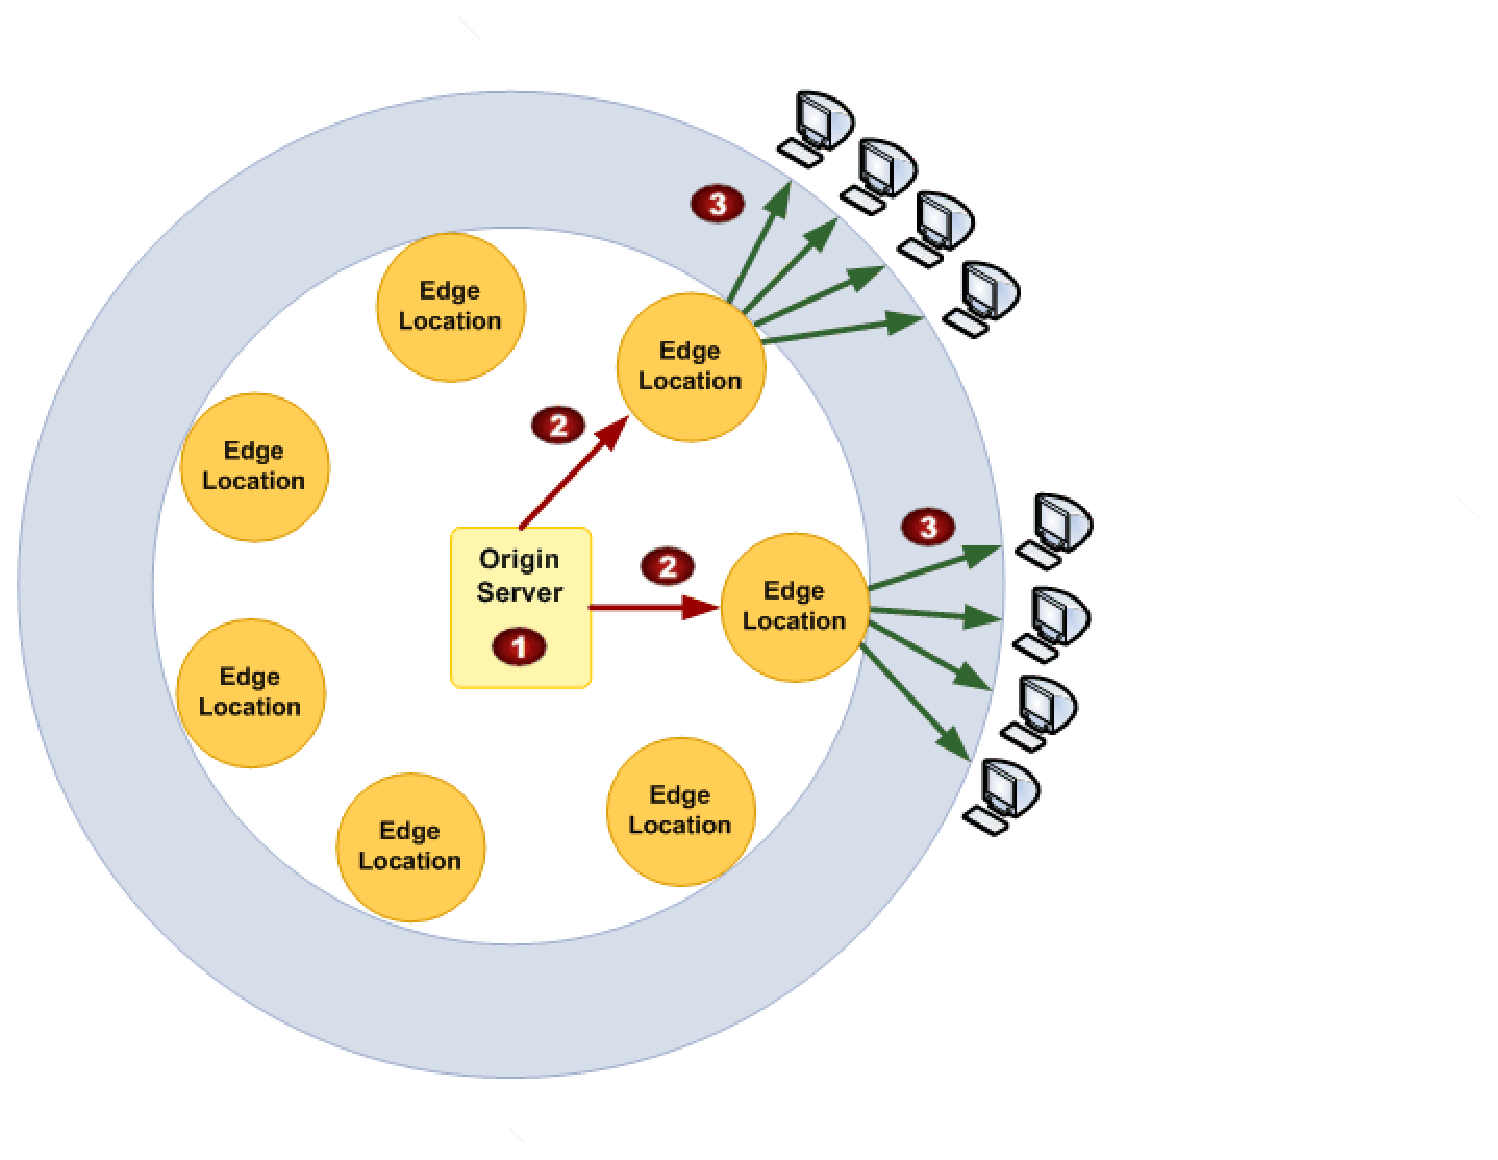
\includegraphics[width= 1.4 \textwidth]{cloudfront.eps}
\end{columns}
\end{frame}
%%%%%%%%%%%%%%%%%%%%%%%%%%%%%%%%%%%%%%%%%%%%%%%%%%%%%%%%%%%%%%%%%%%%%%%%%%%%%%
\begin{frame}
\frametitle[Auto Scaling]{Auto Scaling}
\url{https://aws.amazon.com/autoscaling/}

Auto Scaling allows you to scale your \gls{ec2} capacity up or down automatically according to conditions you define
\begin{itemize}
\item With Auto Scaling, you can ensure that the number of \gls{ec2} instances you’re using increases seamlessly during demand spikes to maintain performance, and decreases automatically during demand lulls to minimize costs
\item Auto Scaling is particularly well suited for applications that experience hourly, daily, or weekly variability in usage
\end{itemize}
\end{frame}
%%%%%%%%%%%%%%%%%%%%%%%%%%%%%%%%%%%%%%%%%%%%%%%%%%%%%%%%%%%%%%%%%%%%%%%%%%%%%%
\begin{frame}
\frametitle[\gls{elb}]{\acrfull{elb}}

\begin{columns}
\column{0.70 \textwidth}
\url{http://aws.amazon.com/elasticloadbalancing/}
\gls{elb}
\begin{itemize}
  \item automatically distributes incoming application traffic across multiple \gls{ec2} instances
  \item enables you to achieve even greater fault tolerance in your applications, seamlessly providing the amount of load balancing capacity needed in response to incoming application traffic
  \item detects unhealthy instances within a pool and automatically reroutes traffic to healthy instances until the unhealthy instances have been restored
\end{itemize}
\column{0.4 \textwidth}
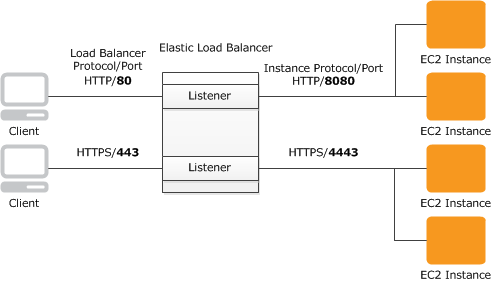
\includegraphics[width=1.0 \textwidth]{elb-listeners.png}
\end{columns}

\end{frame}
%%%%%%%%%%%%%%%%%%%%%%%%%%%%%%%%%%%%%%%%%%%%%%%%%%%%%%%%%%%%%%%%%%%%%%%%%%%%%%
\begin{frame}
\frametitle[Simple DB]{Simple DB}
\url{http://aws.amazon.com/simpledb/}

\begin{itemize}
  \item SimpleDB is a highly available and flexible non-relational data store that offloads the work of database administration
  \item Developers simply store and query data items via web services requests and Amazon SimpleDB does the rest
  \item Unbound by the strict requirements of a relational database, Amazon SimpleDB is optimized to provide high availability and flexibility, with little or no administrative burden
  \item You can change your data model on the fly, and data is automatically indexed for you
\end{itemize}
\end{frame}
%%%%%%%%%%%%%%%%%%%%%%%%%%%%%%%%%%%%%%%%%%%%%%%%%%%%%%%%%%%%%%%%%%%%%%%%%%%%%%
\begin{frame}[fragile, allowframebreaks]
\frametitle[CloudWatch]{CloudWatch}
\url{http://aws.amazon.com/cloudwatch/}

Amazon CloudWatch 
\begin{itemize}
\item provides monitoring for \gls{aws} cloud resources and the applications customers run on \gls{aws}
\item monitors AWS resources such as \gls{ec2} and \gls{rds} instances, and can also monitor custom metrics generated by a customer’s applications and services
\item lets you programmatically retrieve your monitoring data, view graphs, and set alarms to help you troubleshoot, spot trends, and take automated action based on the state of your cloud environment
\end{itemize}
\begin{columns}
\column{0.60 \textwidth}
\begin{center}
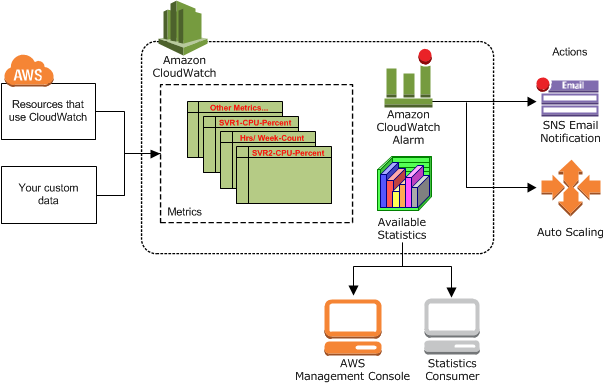
\includegraphics[width=1.0 \textwidth]{CW-Overview.png}
\end{center}
\column{0.45 \textwidth}
\begin{center}
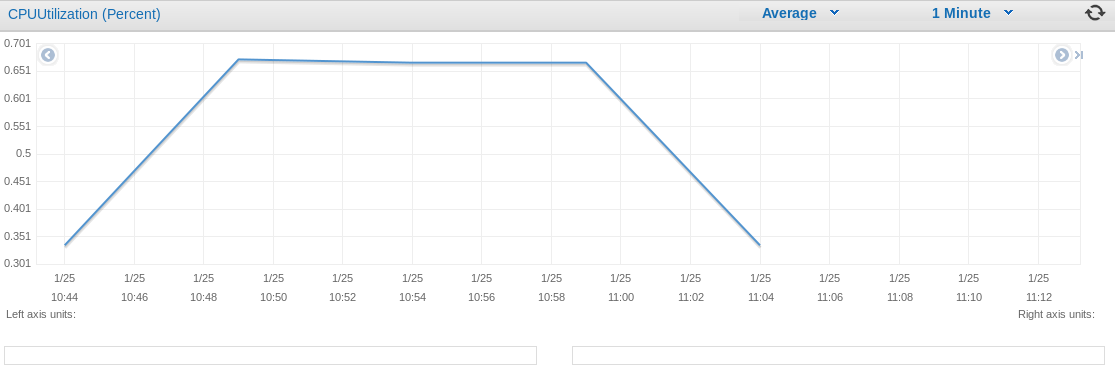
\includegraphics[width=1.0 \textwidth]{cpuutilization.png}
\end{center}
\end{columns}
\end{frame}



%%%%%%%%%%%%%%%%%%%%%%%%%%%%%%%%%%%%%%%%%%%%%%%%%%%%%%%%%%%%%%%%%%%%%%%%%%%%%%
\begin{frame}
\frametitle[\gls{sqs}]{\acrfull{sqs}}

\begin{columns}
\column{0.5 \textwidth}
\url{http://aws.amazon.com/sqs/}
\gls{sqs} 
\begin{itemize}
 \item is a fast, reliable, scalable, fully managed queue service
  \item makes it simple and cost-effective to decouple the components of a cloud application
\end{itemize}
\column{0.50 \textwidth}
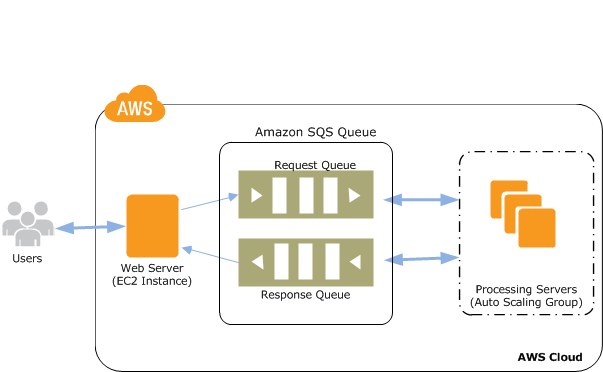
\includegraphics[width=1.0 \textwidth]{sqs-as-workflow.png}
\end{columns}
\end{frame}
%%%%%%%%%%%%%%%%%%%%%%%%%%%%%%%%%%%%%%%%%%%%%%%%%%%%%%%%%%%%%%%%%%%%%%%%%%%%%%
\section{Sign Up Amazon Web Service}
%%%%%%%%%%%%%%%%%%%%%%%%%%%%%%%%%%%%%%%%%%%%%%%%%%%%%%%%%%%%%%%%%%%%%%%%%%%%%%
\begin{frame}[fragile]
\frametitle{Registration in Amazon Web Services}
\begin{itemize}
 \item All you need \dots
 \begin{itemize}
   \item A desktop or laptop (with Internet access, of course)
   \item A credit card (for setting up an AWS account)
   \item A phone (to complete the registration process)
 \end{itemize}
\end{itemize}
\end{frame}
%%%%%%%%%%%%%%%%%%%%%%%%%%%%%%%%%%%%%%%%%%%%%%%%%%%%%%%%%%%%%%%%%%%%%%%%%%%%%%
%%%%%%%%%%%%%%%%%%%%%%%%%%%%%%%%%%%%%%%%%%%%%%%%%%%%%%%%%%%%%%%%%%%%%%%%%%%%%%
\begin{frame}[fragile, allowframebreaks]
\frametitle{Registration in Amazon Web Services}
\begin{itemize}
\item Choose \texttt{Sign Up} button in \url{http://aws.amazon.com/console/} 
\begin{enumerate}
 \item  Create an AWS Account: Login Credentials and Contact Information
  \item Payment Method: Credit Card, Card Number, Cardholder's Name, Expiration Date, Value Added Tax Information
  \item Identity Verification
  \item Support Plan
 \end{enumerate}

\item Sign in!
\item Navigate to Billing and Cost Management, then Credits an introduce de Promotional Code
\begin{center}
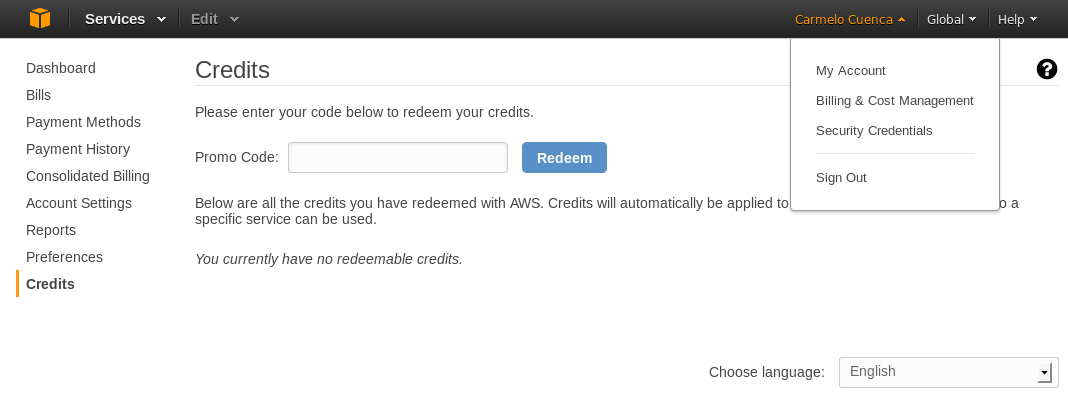
\includegraphics[scale=0.25]{credits.png}
\end{center}
\end{itemize}

\end{frame}
%%%%%%%%%%%%%%%%%%%%%%%%%%%%%%%%%%%%%%%%%%%%%%%%%%%%%%%%%%%%%%%%%%%%%%%%%%%%%%
\end{document}

\section*{Acronyms}
\begin{frame}
\frametitle[Acronyms]{Acronyms}
\glsaddall
\printglossary[type=\acronymtype] % prints just the list of acronyms
\end{frame}
%%%%%%%%%%%%%%%%%%%%%%%%%%%%%%%%%%%%%%%%%%%%%%%%%%%%%%%%%%%%%%%%%%%%%%%%%%%%%%
%%%%%%%%%%%%%%%%%%%%%%%%%%%%%%%%%%%%%%%%%%%%%%%%%%%%%%%%%%%%%%%%%%%%%%%%%%%%%%




